\section{Reasoning in RTEC}\label{sec:reasoning example}

Reasoning has to be efficient enough to support real-time decision-making, and scale to very large numbers of input and output entities. Input entities may not necessarily arrive at RTEC in a timely manner, i.e.~there may be a (variable) delay between the time at which input entities take place and the time at which they arrive at RTEC. Moreover, input entities may be revised, or even completely discarded in the future, as in the case where the parameters of an input entity were originally computed erroneously and are subsequently revised, or in the case of retraction of an input entity that was reported by mistake, and the mistake was realised later.

RTEC performs narrative assimilation by computing and storing the maximal intervals of output entities, i.e.~the intervals of fluents and the time-points in which events occur. Reasoning takes place at specified query times $Q_1, Q_{2}, \dots$. At each $Q_i$ the input entities that fall within a specified interval --- the window $\omega$ --- are taken into consideration. All input entities that took place before or at $Q_i{-}\omega$ are discarded. This is to make the cost of reasoning dependent only on $\omega$ and not on the complete history. The size of $\omega$ and the temporal distance between two consecutive query times --- the slide step $Q_{i}{-}Q_{i-1}$ --- are set by the user. 

At $Q_i$, the output entity maximal intervals computed by RTEC are those that can be derived from the input entities that occurred in the interval $(Q_{i}{-}\omega, Q_{i}]$, as recorded at time $Q_i$. When $\omega$ is longer than the slide step, i.e., when $Q_{i}{-}\omega {<} Q_{i-1} {<} Q_{i}$, it is possible that an input entity occurs in the interval $(Q_{i}{-}\omega, Q_{i-1}]$ but arrives at RTEC only after $Q_{i-1}$; its effects are taken into account at query time $Q_i$. And similarly for input entities that took place in $(Q_{i}{-}\omega, Q_{i-1}]$ and were subsequently revised after $Q_{i-1}$. In the common case that input entities arrive at RTEC with delays, or there is input entity revision, it is preferable therefore to make $\omega$ longer than the slide step. 
Note that information may still be lost. Any input entities arriving or revised between $Q_{i-1}$ and $Q_i$ are discarded at $Q_i$ if they took place before or at $Q_i{-}\omega$. 
To reduce the possibility of losing information, one may increase the size of $\omega$. Doing so, however, decreases recognition efficiency. In what follows we give an example and a detailed account of the `windowing' algorithm of RTEC.

\begin{figure}[t]
	\centering
		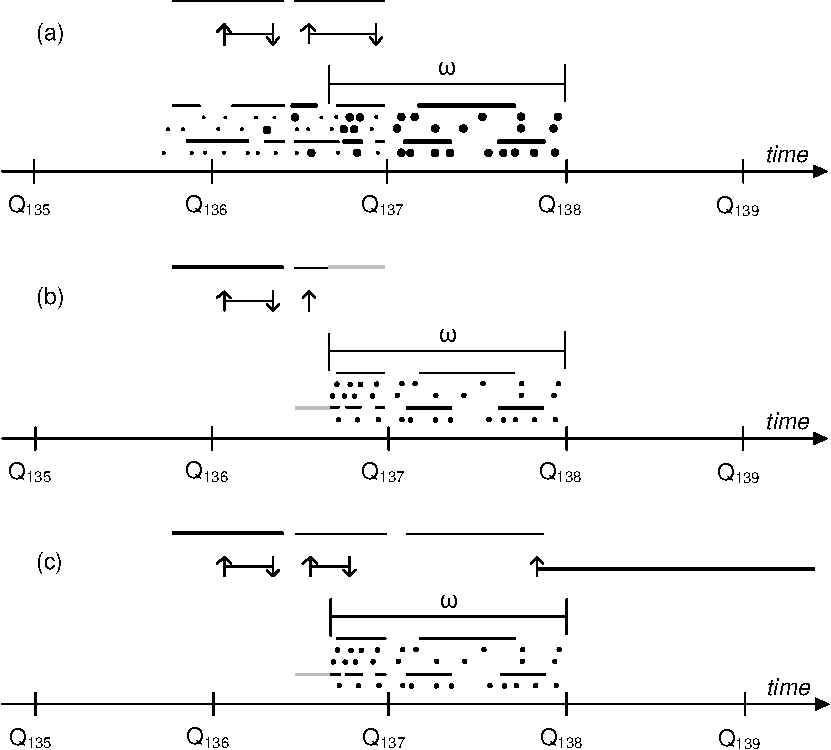
\includegraphics[width=0.6\textwidth]{figures/caching-EC}
	\caption{Windowing in RTEC.}
	\label{fig:rtec-abc}
\end{figure}

Figure \ref{fig:rtec-abc} illustrates windowing in RTEC. In this example we have  $\omega{>}Q_i{-}Q_{i-1}$. To avoid clutter, Figure \ref{fig:rtec-abc} shows streams of only five input entities. These are displayed below $\omega$, with dots for instantaneous input entities and lines for durative ones. For the sake of the example, we are interested in just two fluents:
%
\begin{itemize}
 \item A simple fluent \textttsmall{Se}. The maximal intervals of \textttsmall{Se} are displayed above $\omega$ in Figure \ref{fig:rtec-abc}.
 
 \item A statically determined fluent \textttsmall{Std}. For the example, the maximal intervals of \textttsmall{Std} are defined to be the union of the maximal intervals of the two durative input entities in Figure \ref{fig:rtec-abc}.  The maximal intervals of \textttsmall{Std} are displayed above the \textttsmall{Se} intervals.
\end{itemize}
%
For simplicity, we assume that both \textttsmall{Se} and \textttsmall{Std} are defined only in terms of input entities, i.e.~they are not defined in terms of other output entities.

Figure \ref{fig:rtec-abc} shows the steps that are followed at an arbitrary query time, say $Q_{138}$. Figure \ref{fig:rtec-abc}(a) shows the state of RTEC as computation begins at $Q_{138}$. All input entities that took place before or at $Q_{137}{-}\omega$ were retracted at $Q_{137}$. The thick lines and dots represent the input entities that arrived at RTEC between $Q_{137}$ and $Q_{138}$; some of them took place before $Q_{137}$. Figure \ref{fig:rtec-abc}(a) also shows the maximal intervals for the fluents \textttsmall{Se} and \textttsmall{Std} that were computed and stored at $Q_{137}$.

Reasoning at $Q_{138}$ considers the input entities that took place in $(Q_{138}{-}\omega, Q_{138}]$. All input entities that took place before or at $Q_{138}{-}\omega$ are discarded, as shown in Figure \ref{fig:rtec-abc}(b). For durative input entities that started before $Q_{138}{-}\omega$ and ended after that time, RTEC retracts the sub-interval up to and including $Q_{138}{-}\omega$. Figure \ref{fig:rtec-abc}(b) shows the interval of an input entity that is partially retracted in this way. 

Now consider output entity intervals. At $Q_i$ some of the maximal intervals computed at $Q_{i-1}$ might have become invalid. This is because some input entities occurring in $(Q_i{-}\omega, Q_{i-1}]$ might have arrived or been revised after $Q_{i-1}$: their existence could not have been known at $Q_{i-1}$. Determining which output entity intervals should be (partly) retracted in these circumstances can be computationally very expensive \cite{DBLP:journals/tkde/ArtikisSP15}. We find it simpler, and more efficient, to discard all output entity intervals in $(Q_i{-}\omega, Q_i]$ and compute all intervals from scratch in that period. Output entity intervals that have ended before or at $Q_i{-}\omega$ are discarded. Depending on the user requirements, these intervals may be stored in a database for retrospective inspection of the activities of a system.

In Figure~\ref{fig:rtec-abc}(b), the earlier of the two maximal intervals computed for \textttsmall{Std} at $Q_{137}$ is discarded at $Q_{138}$ since its endpoint is before $Q_{138}{-}\omega$. The later of the two intervals overlaps $Q_{138}{-}\omega$ (an interval `overlaps' a time-point $t$ if the interval starts before or at $t$ and ends after or at that time) and is partly retracted at $Q_{138}$. Its starting point could not have been affected by input entities arriving between $Q_{138}{-}\omega$ and $Q_{138}$ but its endpoint has to be recalculated. Accordingly, the sub-interval from $Q_{138}{-}\omega$ is retracted at $Q_{138}$.

In this example, the maximal intervals of \textttsmall{Std} are determined by computing the union of the maximal intervals of the two durative input entities shown in Figure \ref{fig:rtec-abc}. At $Q_{138}$, only the input entity intervals in $(Q_{138}{-}\omega, Q_{138}]$ are considered. In the example, there are two maximal intervals for \textttsmall{Std} in this period as can be seen in Figure~\ref{fig:rtec-abc}(c). The earlier of them has its start-point at $Q_{138}{-}\omega$. Since that abuts the existing, partially retracted sub-interval for \textttsmall{Std} whose endpoint is $Q_{138}{-}\omega$, those two intervals are amalgamated into one continuous maximal interval as shown in Figure~\ref{fig:rtec-abc}(c). In this way, the endpoint of the \textttsmall{Std} interval that overlapped $Q_{138}{-}\omega$ at $Q_{137}$ is recomputed to take account of input entities available at $Q_{138}$. (In this particular example, it happens that the endpoint of this interval is the same as that computed at $Q_{137}$. That is merely a feature of this particular example. Had \textttsmall{Std} been defined e.g.~as the \emph{intersection} of the maximal intervals of the two durative input entities, then the intervals of \textttsmall{Std} would have changed in $(Q_{138}{-}\omega, Q_{137}]$.)
 

Figure \ref{fig:rtec-abc} also shows how the intervals of the simple fluent \textttsmall{Se} are computed at $Q_{138}$. Arrows facing upwards (downwards) denote the starting (ending) points of the intervals of \textttsmall{Se}. 
First, in analogy with the treatment of statically determined fluents, the earlier of the two \textttsmall{Se}   intervals in Figure~\ref{fig:rtec-abc}(a), and its start and endpoints, are retracted. They occur before $Q_{138}{-}\omega$. The later of the two intervals overlaps $Q_{138}{-}\omega$. The interval is retracted, and only its starting point is kept; its new endpoint, if any, will be recomputed at $Q_{138}$. See Figure \ref{fig:rtec-abc}(b). For simple fluents, it is simpler, and more efficient, to retract such intervals completely and reconstruct them later from their start and endpoints by means of the domain-independent \holdsFor\ rules, rather than keeping the sub-interval that takes place before $Q_{138}{-}\omega$, and possibly amalgamating it later with another interval, as we do for statically determined fluents.
%
%If the last, or any other interval of \textttsmall{Se} that was computed at $Q_{137}$, had started after $Q_{138}{-}\omega$, then the interval and its starting point (and ending point) would have been discarded when the CE recognition process commenced at $Q_{138}$. 
%All ending points after $Q_{138}{-}\omega$, computed at $Q_{137}$, are also discarded.
%

The second step for \textttsmall{Se} at $Q_{138}$ is to calculate its starting and ending points by evaluating the relevant \initiatedAt\ and \terminatedAt\ rules. For this, we only consider input entities that took place in $(Q_{138}{-}\omega, Q_{138}]$. 
Figure \ref{fig:rtec-abc}(c) shows the starting and ending points of \textttsmall{Se} in $(Q_{138}{-}\omega, Q_{138}]$. The last ending point of \textttsmall{Se} that was computed at $Q_{137}$ was invalidated in the light of the new input entities that became available at $Q_{138}$ (compare Figures \ref{fig:rtec-abc}(c)--(a)). Moreover, another ending point was computed at an earlier time.  

Finally, in order to process \textttsmall{Se} at $Q_{138}$ we use the domain-independent \holdsFor\ to calculate the maximal intervals of \textttsmall{Se} given its starting and ending points. The later of the  two \textttsmall{Se} intervals computed at $Q_{137}$ became shorter when re-computed at $Q_{138}$. The second interval of \textttsmall{Se} at $Q_{138}$ is open: given the input entities available at $Q_{138}$, we say that \textttsmall{Se} holds \emph{since} time $t$, where $t$ is the last starting point of \textttsmall{Se}.

The example used for illustration shows how RTEC performs reasoning. In the following section we have a closer look at the operation of RTEC, discussing each of its modules.

